%!TEX program = xelatex

\documentclass[varwidth,convert]{BHCexam1_simple}
\usepackage{gensymb}
\usepackage{mathrsfs}
\usepackage{tikz,pgfplots,float} %绘图
\usepackage{tkz-euclide}
\usepackage{graphicx}
\usepackage{wrapfig}
\usepackage[english]{babel}
\usepackage{caption}
\usepackage{CJK}
\usepackage{enumitem}
\usetikzlibrary{calc,quotes,angles,babel,intersections,arrows,automata,positioning}

\pgfplotsset{compat=1.15}
\tikzset{ 
  right angle quadrant/.code={ 
   \pgfmathsetmacro\quadranta{{1,1,-1,-1}[#1-1]} % Arrays for selecting quadrant 
   \pgfmathsetmacro\quadrantb{{1,-1,-1,1}[#1-1]}}, 
  right angle quadrant=1, % Make sure it is set, even if not called explicitly 
  right angle length/.code={\def\rightanglelength{#1}}, % Length of symbol 
  right angle length=2ex, % Make sure it is set... 
  right angle symbol/.style n args={3}{ 
   insert path={ 
   let \p0 = ( $(#1)!(#3)!(#2)$ ) in % Intersection 
    let \p1 = ( $(\p0)!\quadranta*\rightanglelength!(#3)$ ), % Point on base line 
    \p2 = ( $(\p0)!\quadrantb*\rightanglelength!(#2)$ ) in % Point on perpendicular line 
    let \p3 = ( $(\p1)+(\p2)-(\p0)$ ) in % Corner point of symbol 
   (\p1) -- (\p3) -- (\p2) 
   } 
  } 
}

\setlength{\textwidth}{20cm}

\begin{document}

%%% -------- Anchor Start -------- %%%

已知长方形$ABCO$,~$O$为坐标原点,点$B$的坐标为$(8,6)$,~$A,C$分别在坐标轴上,$P$是线段$BC$上动点,设$PC=m$,已知点$D$在第一象限且是直线$y=2x+6$上的一点,若$\triangle APD$是等腰直角三角形。
\begin{enumerate}[label={(\arabic*)}]
\item 求点$D$的坐标;
\item 直线$y=2x+6$向右平移6个单位后,在该直线上,是否存在点$D$,使$\triangle APD$是等腰三角形?若存在,请求出这些点的坐标;若不存在,请说明理由。
\end{enumerate}

% \hskip 50pt
\hfill
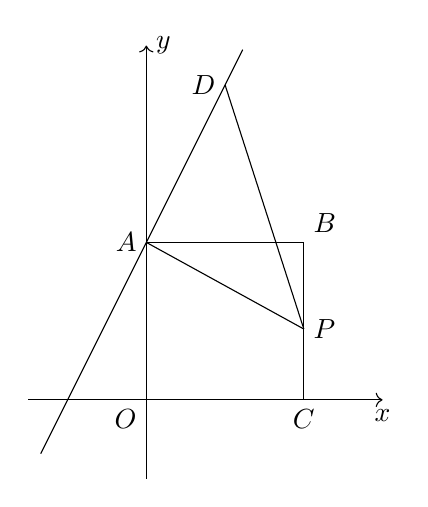
\begin{tikzpicture}[dot/.style={circle,inner sep=1pt,fill,label={#1},name=#1},
 extended line/.style={shorten >=-#1,shorten <=-#1},
 extended line/.default=1cm] %[scale=0.6]
\coordinate [label= below left:$O$] (O) at (0,0);
\coordinate [label= below:$C$] (C) at (2,0);
\coordinate [label= left:$A$] (A) at (0,2);
\coordinate [label= above right:$B$] (B) at (2,2);
\coordinate [label= left:$D$] (D) at (1,4);
\coordinate [label= right:$P$] (P) at($(B)!0.55!(C)$);
\draw [extended line,shorten >=-0.5cm,shorten <=-3cm] (A) -- (D);
\draw (A) -- (B);
\draw (B) -- (C);
\draw (D) -- (P);
\draw (A) -- (P);
\draw [->] (O)+(-1.5,0) -- (3,0) node [below]{$x$};
\draw [->] (O)+(0,-1) -- (0,4.5) node [right]{$y$};
\end{tikzpicture}

%%% -------- Anchor End ---------- %%%

\end{document}